\chapter{Introducción}
\label{sec:introduccion}

\section{Objetivos}

El objetivo del trabajo práctico es lograr un conocimiento práctico en el cálculo y la simulación de circuitos
acondicionadores de señal (CAS). Un CAS adapta la señal eléctrica entregada por un sensor al rango de entrada de un
conversor analógico-digital (A/D), para lo cual por lo general debe amplificar el nivel de tensión del sensor y
realizar un desvío de nivel (\textit{offset}).

\section{Descripción del Trabajo Práctico}

Se diseña un CAS que adapta la señal de un sensor de temperatura LM335 a la entrada del conversor A/D de un
microcontrolador. El trabajo se limita al cálculo de los componentes y a la verificación del comportamiento del
circuito mediante simulación en KiCad (ngspice), sin implementación física. La Figura~\ref{fig:diagrama_bloques}
muestra el diagrama en bloques del sistema.

\begin{figure}[!ht]
  \centering
  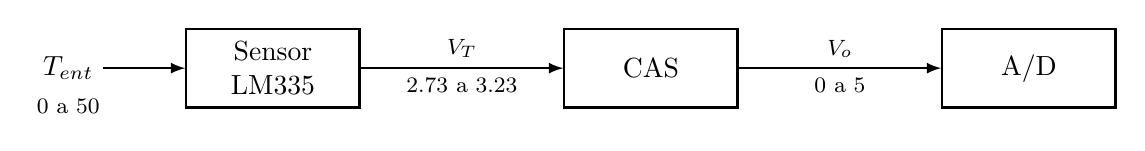
\begin{tikzpicture}[
    bloque/.style={draw, thick, minimum width=2.2cm, minimum height=1cm, align=center},
    >=latex
  ]
  \node (tin) at (0,0) {$T_{ent}$};
  \node[bloque] (sen) at (2.6,0) {Sensor\\LM335};
  \node[bloque] (cas) at (7.4,0) {CAS};
  \node[bloque] (adc) at (12.2,0) {A/D};
  \draw[->, thick] (tin) -- (sen);
  \draw[->, thick] (sen) -- node[above, font=\footnotesize]{$V_T$}
    node[below, font=\footnotesize]{$\SI{2.73}{\volt}$ a $\SI{3.23}{\volt}$} (cas);
  \draw[->, thick] (cas) -- node[above, font=\footnotesize]{$V_o$}
    node[below, font=\footnotesize]{$\SI{0}{\volt}$ a $\SI{5}{\volt}$} (adc);
  \node[below, font=\footnotesize] at (tin.south) {\SI{0}{\celsius} a \SI{50}{\celsius}};
\end{tikzpicture}

  \caption{Diagrama en bloques del sistema de medición.}
  \label{fig:diagrama_bloques}
\end{figure}

\section{Requerimientos de Diseño}

\begin{itemize}
  \item Rango de medición de temperatura: \SI{0}{\celsius} a \SI{50}{\celsius}.
  \item Rango de entrada del conversor A/D: \SI{0}{\volt} a \SI{5}{\volt}.
  \item A \SI{0}{\celsius} debe corresponder $V_o = \SI{0}{\volt}$ y a \SI{50}{\celsius}, $V_o = \SI{5}{\volt}$.
  \item Alimentación simple de \SI{5}{\volt}, la misma del microcontrolador.
\end{itemize}

El LM335 entrega una tensión proporcional a la temperatura absoluta:
\begin{equation}
  V_T = \SI{10}{\milli\volt/\kelvin} \cdot T\,[\unit{\kelvin}]
  \quad\Rightarrow\quad
  V_T = \SI{10}{\milli\volt/\celsius} \cdot T\,[\unit{\celsius}] + \SI{2.73}{\volt}
  \label{eq:sensor}
\end{equation}
por lo que el rango de temperatura corresponde a una tensión del sensor entre $\SI{2.73}{\volt}$ y
$\SI{3.23}{\volt}$.
